\documentclass[11pt,letterpaper]{article}
\usepackage[lmargin=1in,rmargin=1in,tmargin=0.75in,bmargin=1in]{geometry}

% -------------------
% Packages
% -------------------
\usepackage{
	amsmath,			% Math Environments
	amssymb,			% Extended Symbols
	enumerate,		% Enumerate Environments
	graphicx,			% Include Images    
	lastpage,			% Reference Lastpage
	multicol,			% Use Multi-columns
	multirow,			% Use Multi-rows
	siunitx
}

\graphicspath{{./images/}}

\usepackage{wrapfig}

% -------------------
% Font
% -------------------
\usepackage[T1]{fontenc}
\usepackage{charter}    


% -------------------
% Heading Commands
% -------------------
\thispagestyle{empty}
\vspace*{-0.5in}

% -------------------
% Commands
% -------------------

\newcommand{\pspace}{\par\vspace{\baselineskip}}
\newcommand{\ds}{\displaystyle}

% -------------------
% Content
% -------------------

\begin{document}
\begin{minipage}{\textwidth}
     \begin{center}
          \textbf{\huge Mathcounts Sheet}
          \vspace{0.1in}
     \end{center}
\end{minipage} \\
\rule[2ex]{\textwidth}{2pt} 
\centering
\begin{minipage}{\textwidth}
     \noindent \textbf{Test Taking Strategies}
     \begin{itemize}
          \item Be sure to always make an attempt
          \item Don't be afraid to skip a question and return later
          \item Substitute in answer choices
          \item Use smaller cases to find a pattern
          \item Use tools
          \begin{itemize}
               \item Rulers, compasses, and protractors can be used to draw and estimate lengths/angle measures. Diagrams in problems are not drawn to scale.
               \item Use graph paper to model equations to determine possible solutions
          \end{itemize}
          \item Eliminate incorrect answers
          \begin{itemize}
               \item Narrow down possible answers
               \item Increases probability of guesswork
          \end{itemize}
          \item Last resort is to guess
          \begin{itemize}
               \item NEVER LEAVE A QUESTION BLANK, there is no penalty for incorrect answers
          \end{itemize}
     \end{itemize}

\end{minipage}


\vspace{0.4cm}

\begin{minipage}{\textwidth}
     \noindent \textbf{Geometry}
     \begin{center}
          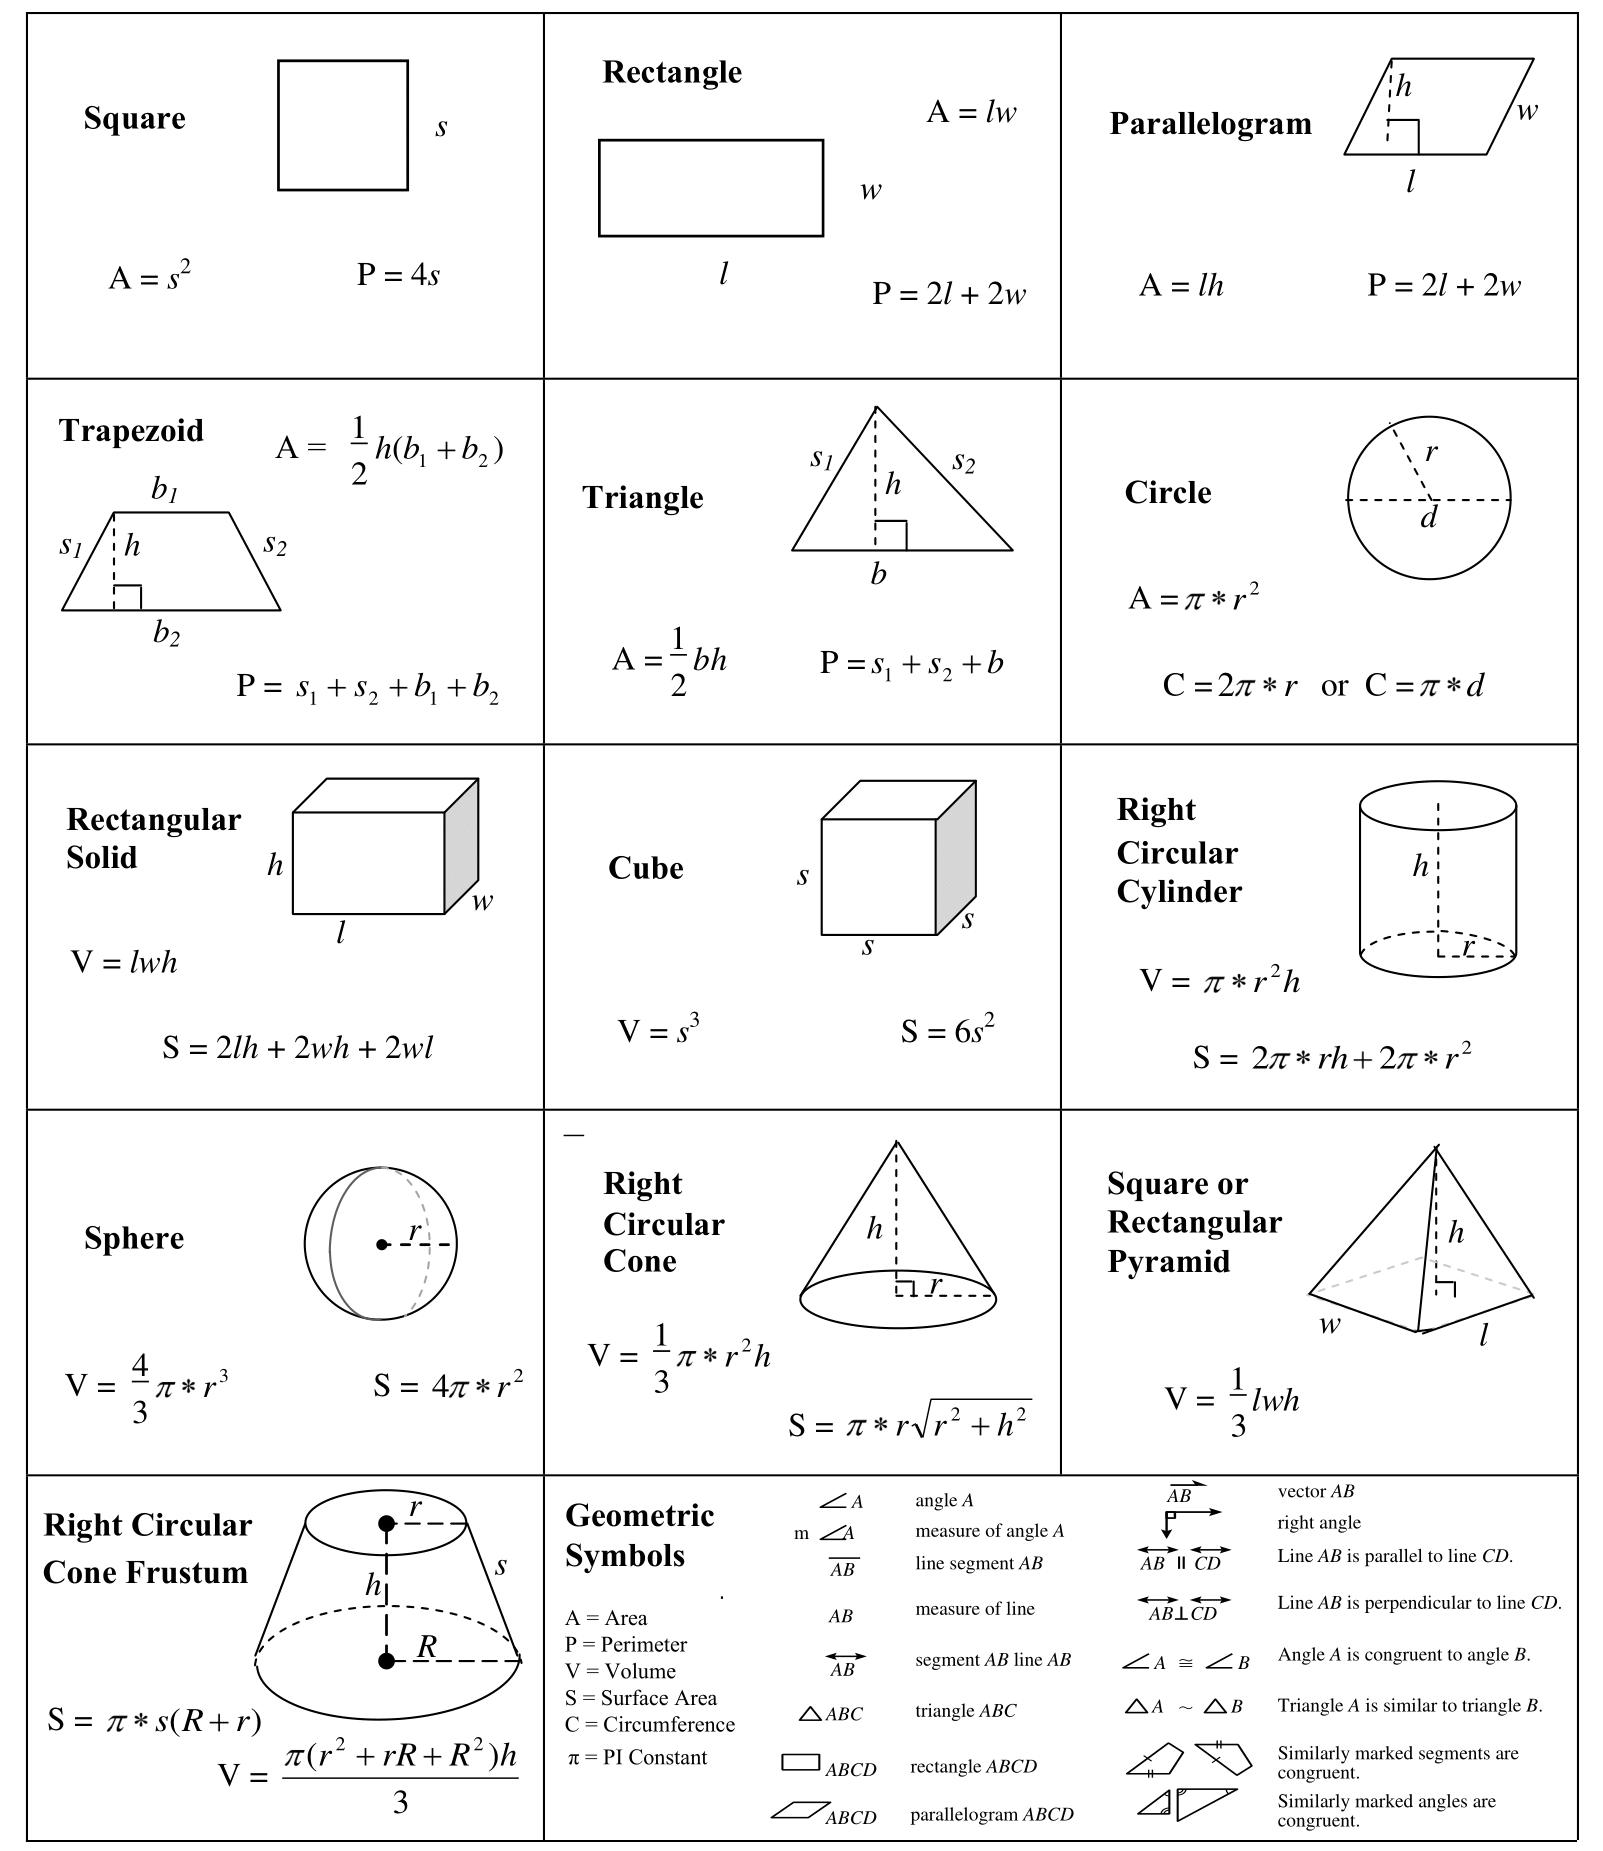
\includegraphics[height = 13cm]{images/geometry.png}
     \end{center}    
\end{minipage}

\vspace{15cm}

\begin{minipage}{\textwidth}
     \begin{itemize}
          \item Angle Pair Relationships
          \begin{itemize}
               \item Adjacent Angles: angles that neighbor each other bisected by a single line
               \item Complementary Angles: angles that add up to $90^{\circ}$
               \item Supplementary/Linear Angle Pairs: angles that add up to $180^{\circ}$ along a straight line
               \item Vertical Angles: pairs of opposite angles made by two intersecting lines
               
               \vspace{0.2cm}
               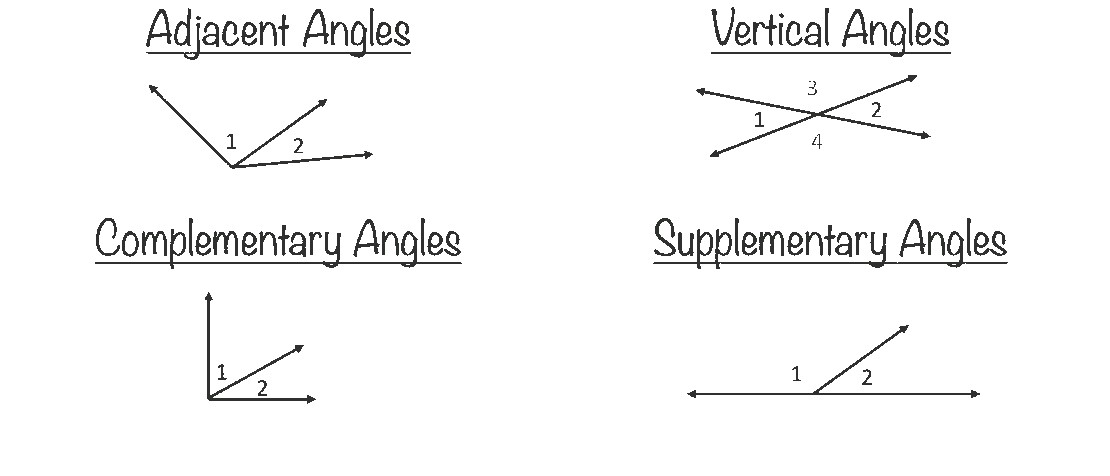
\includegraphics[height = 7cm]{images/anglrel.jpg}
          \end{itemize}
          \vspace{-0.5cm}
          \item Triangles
          \begin{itemize}
               \item When a triangle has an angle of $90^{\circ}$, the sum of the squared legs is equal to the squared hypotenuse; $a^2+b^2=c^2$
               \item The numbers that are possible for the values of $a$, $b$, and $c$ are known as pythagorean triples. Common triples include:
               \begin{itemize}
                    \item $3$, $4$, $5$
                    \item $5$, $12$, $13$
                    \item $6$, $8$, $10$
                    \item $7$, $24$, $25$
                    \item $9$, $12$, $15$
               \end{itemize}
          \end{itemize}
          \item Circles
          \begin{itemize}
               \item Area of a Sector = $\frac{\pi r^2\theta}{360^{\circ}}$
               \item Length of an Arc = $\frac{2\pi r\theta}{360^{\circ}}$
          \end{itemize}
          \item Polygons
          \begin{itemize}
               \item Sum of the Interior Angles of a Polygon = $(\text{number of sides}-2) * 180$
               \item Measure of an Interior Angle of a Regular Polygon = $\frac{n-2}{n} * 180$
               \item Measure of an Exterior Angle of a Regular Polygon = $\frac{360}{n}$
          \end{itemize}
        \end{itemize} 
\end{minipage}

\vspace{0.4cm}

\begin{minipage}{\textwidth}
     \noindent \textbf{Common Situations/Vocabulary}
     \begin{itemize}
          \item Mean: the average value for a data set = $\frac{\text{Sum of all Terms}}{\text{Number of Terms}}$
          \item Median: the point in the middle of a data set; exactly 1/2 on either side
          \item Mode: the most common number in a data set
          \item Speed: $\frac{Distance}{Time}$
          \item Distance: $Speed * Time$
          \item Combinations: formula to choose $k$ objects from $n$ =${{n}\choose{k}} = \frac{n!}{k!(n-k)!}$
     \end{itemize}
\end{minipage}

\begin{minipage}{\textwidth}
     \vspace{0.4cm}
     \noindent \textbf{Systems of Equations}\\
     A system of equations is a set of equations which share the same variables. Below is an example of a system of equations.
     \begin{itemize}
          \item Elimination
          \begin{itemize}
               \item  Elimination involves removing variables from the system by adding constant multiples of two or more of the equations together.

               \subsection*{Example}
               Find the ordered pair $(x,y)$ for which
               
               \[\left\{\begin{array}{l}x-12y=2\\3x+6y=6\end{array}\right.\]
               \subsection*{Solution}
               We can eliminate $y$ by adding two times the second equation to the first:
               
               $x - 12y + 2(3x+6y)= 2 + 2(6)$
               \\
               Simplifying
               \\${7x + 0=14}$.
               \\
               So, $x=2$. Then, we can plug in for $x$ in either of the equations:\begin{align*} (2)-12y &= 2 \\ y &= 0 \end{align*}
               Thus, the solution to the system is $(2,0)$.
          \end{itemize}
          \item Substitution
          \begin{itemize}
               \item Substitution requires solving for a variable and then plugging that variable into another equation, therefore reducing the number of variables.

               \subsection*{Example}
               Find the ordered pair $(x,y)$ for which
               
               \[\left\{\begin{array}{l}x-12y=2\\3x+6y=6\end{array}\right.\]
               \subsection*{Solution}
               Solving the first equation for x:
               \\ $x = 12y + 2.$
               \\
               Plugging this into the second equation:
               
               $3(12y + 2) + 6y = 6 \Leftrightarrow 42 y = 0.$
               \\
               Thus, $y=0$. Plugging this into either equation and solving for $x$ yields $x=2$.
          \end{itemize}
     \end{itemize}
\end{minipage}
\vspace{0.4cm}
\begin{minipage}{\textwidth}
     \noindent \textbf{Sum of Geometric Sequences}
     \begin{itemize}
          \item A geometric sequence, sometimes called a geometric progression, is a sequence of numbers such that the ratio between any two consecutive terms is constant. This constant is called the common ratio of the sequence.
          \begin{itemize}
               \item For example, $1, 2, 4, 8$ is a geometric sequence with common ratio $2$ and $100, -50, 25, -25/2$ is a geometric sequence with common ratio $-1/2$; however, $1, 3, 9, -27$ and $-3, 1, 5, 9, \ldots$ are not geometric sequences, as the ratio between consecutive terms varies.
               \item More formally, the sequence $a_1, a_2, \ldots , a_n$ is a geometric progression if and only if $a_2 / a_1 = a_3 / a_2 = \cdots = a_n / a_{n-1}$. A similar definition holds for infinite geometric sequences. It appears most frequently in its three-term form: namely, that constants $a$, $b$, and $c$ are in geometric progression if and only if $b / a = c / b$.
          \end{itemize}
          \item Finite
          \begin{itemize}
               \item A finite geometric series with first term $a_1$, common ratio $r$ not equal to one, and $n$ total terms has a value equal to $\frac{a_1(r^n-1)}{r-1}$.
          \end{itemize}
          \item Infinite 
          \begin{itemize}
               \item An infinite geometric series converges if and only if $|r|<1$; if this condition is satisfied, the series converges to $\frac{a_1}{1-r}$.
          \end{itemize}
     \end{itemize}
\end{minipage}
\begin{minipage}{\textwidth}
     \noindent \textbf{Guessing Strategies}
     \begin{itemize}
          \item Sometimes you can eliminate
          \begin{itemize}
               \item Answer choices too large or small
               \item Answer choices odd or even
               \item Answer choices divisible by $x$
          \end{itemize}
          \item In geometry problems, estimate the dimensions
          \begin{itemize}
               \item Graph paper, rulers, and protractors are allowed; draw your own diagrams!
               \item Divide the shape into subsections and estimate the values of each portion
          \end{itemize}
        \end{itemize}
\end{minipage}

\end{document}
